% Created 2017-01-18 Wed 12:52
% Intended LaTeX compiler: pdflatex
\documentclass[11pt]{article}
\usepackage[utf8]{inputenc}
\usepackage{lmodern}
\usepackage[T1]{fontenc}
\usepackage{fixltx2e}
\usepackage{graphicx}
\usepackage{longtable}
\usepackage{float}
\usepackage{wrapfig}
\usepackage{rotating}
\usepackage[normalem]{ulem}
\usepackage{amsmath}
\usepackage{textcomp}
\usepackage{marvosym}
\usepackage{wasysym}
\usepackage{amssymb}
\usepackage{amsmath}
\usepackage[version=3]{mhchem}
\usepackage[numbers,super,sort&compress]{natbib}
\usepackage{natmove}
\usepackage{url}
\usepackage{minted}
\usepackage{underscore}
\usepackage[linktocpage,pdfstartview=FitH,colorlinks,
linkcolor=blue,anchorcolor=blue,
citecolor=blue,filecolor=blue,menucolor=blue,urlcolor=blue]{hyperref}
\usepackage{attachfile}
\usepackage[letterpaper, portrait, margin=1in]{geometry}
\author{Rebecca Taylor}
\date{\today}
\title{Weekly Report}
\begin{document}

\maketitle{}

\section{Project goals for week/month}
\label{sec:orga7c2e54}

Please provide brief description of your research projects. If you have a list of goals or questions, document them as a list:
\begin{itemize}
\item experiment or question 1
\item experiment or question 2
\item experiment or question 3
\end{itemize}

\section{Experiments conducted}
\label{sec:org1664e6f}

Describe the experiments you did this past week.

\subsection{Bex Blurb on Research Ethics}
\label{sec:org1d7926e}
The manner in which you conduct yourselves and your research is as important as the research itself. In order for the community to trust your work, they must be able to trust that you are an ethical person. Take a look in your "At the Bench" books and read the sections on laboratory conduct and research ethics.

Here are links to CMU ethics resources which CMU refers to the "Responsible Conduct of Research". \url{http://www.cmu.edu/research-compliance/responsible-conduct/}
Here is the U.S. Department of Health and Human Services website for the The Office of Research Integrity: \url{https://ori.hhs.gov/ori-introduction-responsible-conduct-research}
And here is a PDF of that website's contents: \url{https://ori.hhs.gov/sites/default/files/rcrintro.pdf}

\section{Data and figures in progress}
\label{sec:orgf559ff0}

Did you make progress? Learn useful lessons? Did it not work? Tell me what you think happened.

If you have data, can you plot it or include an image as a figure? Here is an example showing you how to insert a figure that is a PNG file:

\begin{figure}[htbp]
\centering
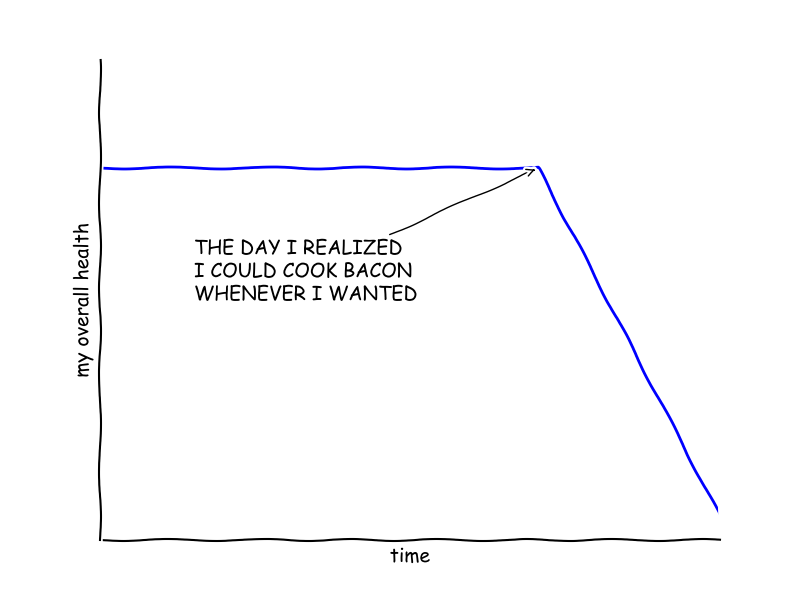
\includegraphics[width=4in]{JohnKitchinBacon.png}
\caption{\label{fig:1}
John Kitchin's XKCD-style bacon plot}
\end{figure}

Note: In true LaTex style, the figure shows up where there is space for it at the top of the next page.

\section{New papers of interest}
\label{sec:orgdfbe2d6}

Describe 1 or 2 notable papers that you read this week. Include citations for them so that you can build your personal database of relevant papers and be ready to cite them in your future publications. For example, say you stumbled across Bex's stretchable microelectrode array paper \cite{Taylor2013JMM}.

You should watch John Kitchin's screencast that describes how org-ref works. This will teach you have to create references using the key binding "Ctrl-C ]". Here is the link: \url{http://www.screencast.com/t/bxfafVydE}. For now I recommend you use org-ref just for your bibliographies and later you can explore org-ref for linking to figures and tables and document sections.

\bibliography{TaylorLab-publications}
\bibliographystyle{abbrv}

\label{bibliography}
\end{document}
